\section{The Common\-Collector BJT Amplifier}

\subsection{Experiment Design}
    \subsubsection{Background}
    An Amlifier is a device that can increase the power of a signal.
    And a Common\-Collector BJT Amplifier have the characters of high input impedance and low output impedance.
    It can be used as a buffer to isolate the input and output impedance of the circuit.\par

    \subsubsection{Propose}
    \begin{itemize}
        \item Measure the quiescent-point of an emitter follwer(CC Amplifier)
        \item Ecaluate the small-signal amplification function of an emitter follower
    \end{itemize}

\subsection{Experiment Design}
    \subsubsection{Materials}
        In this experiment, we will use the following components:
        \begin{itemize}
            \item 2N3904\_1
            \item Capacitors
            \item Resistors
            \item DC Power Supply
            \item Function Generator
            \item Oscilloscope
            \item Digital Multimeter
        \end{itemize}
    \subsubsection{Circuit Diagram}
        The circuit diagram of the Common\-Collector BJT Amplifier is shown in Figure \ref{fig:CC_Amplifier}.
        \begin{figure}[H]
            \centering
            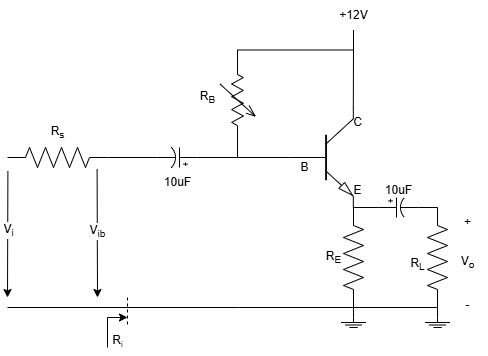
\includegraphics[width=0.5\linewidth]{Experiment_07/Circuit/Lab7.drawio.png}
            \caption{Common\-Collector BJT Amplifier}
        \end{figure}

    \subsubsection{Theoretical Analysis}

    \begin{enumerate}[I]
        \item \textbf{DC Analysis}
            First, we analyze the circuit by drawing its DC-equivalent circuit to find its quiescent working point.\par
            \begin{figure}[H]
                \centering
                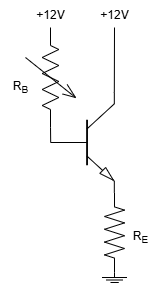
\includegraphics[width=0.2\linewidth]{Experiment_07/Circuit/Lab7dc.drawio.png}
                \caption{DC-equivalent Circuit}
                \label{cir:7dc}
            \end{figure}
            In Fig.\ref{cir:7dc}, we can obtain the expression of some basic current.
            \begin{equation}
                V_{CC} - i_B R_B - V_{BE} - (1+\beta) i_B R_E = 0, \quad
                i_B = \frac{V_{CC} - V_{BE}}{R_B + (1+\beta) R_E}     
            \end{equation}
        \item \textbf{AC Analysis}
            Next, we analyze the circuit by drawing its AC-equivalent circuit to find its small-signal amplification function.\par
            \begin{figure}[H]
                \centering
                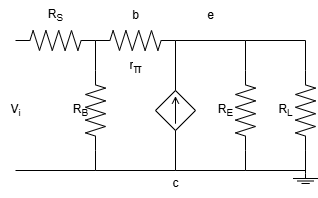
\includegraphics[width=0.5\linewidth]{Experiment_07/Circuit/Lab7ac.drawio.png}
                \caption{AC-equivalent Circuit}
                \label{cir:7ac}
            \end{figure}
            In Fig.\ref{cir:7ac}, we can obtain the expression of the voltage gain, input impedance, and output impedance.
            \begin{itemize}
                \item \textbf{Input output voltage:}
                \[
                    V_o = (R_E \parallel R_L)(1+\beta) i_B, \quad
                    V_i = i_B r_\pi + V_o + R_S \left(i_B + \frac{i_B r_\pi + V_o}{R_B}\right)
                \]
                \item \textbf{Voltage gain:}
                \[
                    A_V = \frac{V_o}{V_i}
                \]
                \item \textbf{Input and Output impedance:}
                \[
                    R_i = \frac{i_B r_\pi + V_o}{\frac{i_B}{R_B} + \frac{1}{R_S}}, \quad
                    R_o = \frac{V_x}{i_x}
                \]
                where $V_x$ and $i_x$ is given by the following equation:
                \[
                    I_x + (1+\beta)i_B = \frac{V_x}{R_E \parallel R_L}, \quad
                    V_x + i_B r_\pi + i_B(R_S \parallel R_B)
                \]
            \end{itemize}
    \end{enumerate}

\subsection{Experiment record}
\subsubsection{DC Analysis}
Set $v_i$ as zero, and we can measure the terminal voltage of the BJT\\
    \begin{equation}
    \centering
            V_B =10.10,\quad
            V_C =12.00,\quad
            V_E =9.505
            \label{eq:7demeas}
    \end{equation}
    Plug equation \ref{eq:7demeas} into the theoretical euquation we obtained above, we can obtain:

        \begin{align*}
            I_{BQ} & = \frac{V_C-V_B}{R_B}=33.929\mu A\\
            I_{EQ} & = \frac{V_E}{R_E}=9.505mA\\
            I_{CQ} & = I_{EQ}-I_{BQ}=9.471mA\\
            \beta  & = 279.14
        \end{align*}


\subsubsection{AC Analysis}
\begin{itemize}
    \item Voltage Gain: Let $v_i$ to be a sinusoidal signal (1000 Hz, 5V peak) and $R_L$ = 300k$\Omega$.
        \begin{table}[h]
        \centering
        \begin{tabular}{l|cccc}
            \toprule
            Vib & 0.9372     & 0.7239      & 0.4901    & 0.24     \\ 
            Vo  & 0.9425     & 0.7072      & 0.4824    & 0.2411   \\
            \midrule
            Av  & 1.00565514 & 0.976930515 & 0.9842889 & 1.004583 \\ 
            \bottomrule
        \end{tabular}
        \caption{Voltage Gain}
        \end{table}
        \FloatBarrier
        When the BJT turns to saturation, the distortion occurs. $R_B$ should be increased to enlarge the linear amplification range.
    \item Input \& Output Resistance: Let $v_i$ to be  a 1000 Hz sinusoidal signal with the amplitude of 1 V.
        The input and output resistance is calculated as the following:
        \begin{equation}
            R_i = \frac{v_{ib} R_S}{v_i-v_{ib}} = \frac{10K * 0.578}{1.15 - 0.578} = 10104.9\Omega
        \end{equation}

        
\end{itemize}

        %\item \textbf{Real Output Impedance}\par
        %    First, we assumet the open-circuit voltage gain is $V_{oc}$, then, we can write the output voltage with load as the following:
        %    \begin{equation}
        %            V_{L1} = V_{OC} \cdot \frac{R_{L1}}{Z_{out} + R_{L1}}
        %    \end{equation}
        %    \begin{equation}
        %            V_{L2} = V_{OC} \cdot \frac{R_{L2}}{Z_{out} + R_{L2}}
        %    \end{equation}
        %    Then, we can get emilate the $V_{oc}$, and find the expression of the output impedance as the following:
        %    \begin{equation}
        %        Z_{out} = \frac{R_{L1} \cdot R_{L2} \cdot (V_{L1} - V_{L2})}{V_{L2} \cdot R_{L1} - V_{L1} \cdot R_{L2}}
        %    \end{equation}

        %    Substitude the value of $V_{L1}$ and $V_{L2}$ for resistance $300k\Omega$ and $1k\Omega$ we can calculate the real output impedance of the circuit:

        %    \begin{equation}
        %        Z_{out} = \frac{300k\Omega \cdot 1k\Omega \cdot (0.588V - 0.568V)}
        %                       {0.568V \cdot300k\Omega -0.588V \cdot 1k\Omega}
        %                = 
        %    \end{equation}
\subsection{Experiment Conclusion}
    \subsubsection{Conclusion}
    In this experiment, we have successfully measured the quiescent-point of an emitter follower(CC Amplifier) and ecaluated the small-signal amplification function of an emitter follower.
    
